\iffalse\documentclass{article}\fi
\documentclass[12pt]{article}

\usepackage{sbc-template}
\usepackage{graphicx,url}

%sudo apt install texlive-lang-portuguese
\usepackage[portuguese]{babel}   
\usepackage[utf8]{inputenc} 

\usepackage{graphicx}

%\usepackage[numbib,nottoc]{blindtext}
%\usepackage[numbib,nottoc]{tocbibind}

\graphicspath{ {./images/} }

\sloppy

\title{Avaliação de superpixels para segementação de imagens}

%Avaliar se superpixels podem ser utilizadas na segmentação de imagens sem diminuição do desempenho da segmentação, porém com custo inferior.

\author{Felipe Augusto Lima Reis\inst{1}}

\address{PUC Minas - Pontifícia Universidade Católica de Minas Gerais
  \email{falreis@sga.pucminas.br} }

\begin{document} 

\maketitle

\begin{abstract}
  Superpixels are structures that group similar pixels into sets that reflect aspects of the image. This article evaluates the use of SLICO superpixels and partition hierarchy for segmentation. Using \textbf{neural networks} for segmentation, the results of superpixels images with different levels of granularity and untreated images were compared to the ground-truth. The article also evaluates the training time of neural networks for superpixels based images. For training and evaluation, the Berkeley Segmentation Data Set (BSDS500) \cite{BSDS500} image was used.
\end{abstract}
     
\begin{resumo} 
  Superpixels são estruturas que agrupam pixels semelhantes em conjuntos que refletem aspectos da imagem. Este artigo avalia a utilização superpixels SLICO e hierarquia de partições para segmentação. Utilizando \textbf{redes neurais} para segmentação, os resultados de imagens utilizando superpixels com diferentes níveis de granularidade e imagens sem tratamento foram comparadas em relação ao \textit{ground-truth}. O artigo também avalia o tempo de treinamento das redes neurais para imagens com superpixels em relação às imagens originais. Para treinamento e avaliação foram utilizadas imagem do Berkeley Segmentation Data Set (BSDS500) \cite{BSDS500}.
\end{resumo}


\section{Introdução} \label{sec:introducao}

A segmentação de imagens consiste em dividir uma imagem em um conjunto de regiões logicamente agrupadas, de modo a reunir áreas que contém informação relevante dentro dos grupos \cite{DOMINGUEZ}. Nessa tarefa, tomamos os \textit{pixels} como unidades básicas de processamento \cite{WANG201728}. O agrupamento de pixels em unidades maiores permite um tipo de segmentação chamado de \textit{oversegmentation} \cite{WANG201728}, ilustrada na figura \ref{fig:superpixel}. O uso de superpixels possibilita o aumento da velocidade de processamento posterior, uma vez que a quantidade de pixels diminui consideravelmente em relação a imagem original.

\begin{figure}[ht]
\centering
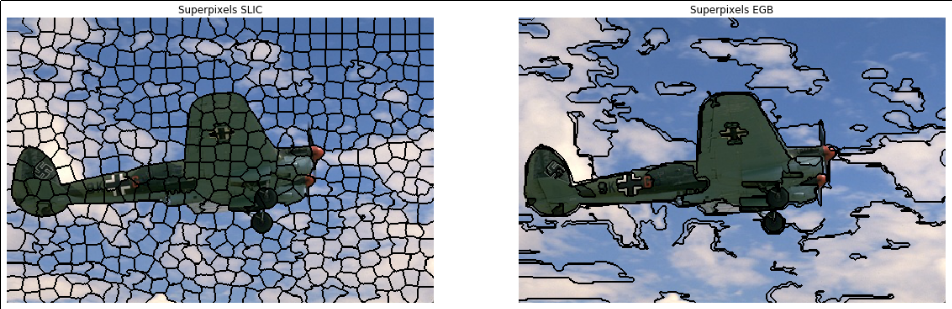
\includegraphics[width=1.\textwidth]{superpixels.png}
\caption{Imagem segmentada utilizando superpixel SLIC, com aproximadamente 500 segmentos.}
\label{fig:superpixel}
\end{figure}

A utilização de superpixels possibilita a redução de itens a serem processados, entretanto pode causar perda de informação importante. No entanto, para alguns casos, a perda de qualidade pode se justificar em relação ao ganho de velocidade obtido utilizando esse tipo de operação. Essa relação consiste então em um \textit{trade-off} entre ambas as características, sendo viáveis em alguns cenários de processamento em tempo real ou para dispositivos com baixo desempenho.

O presente trabalho tem como objetivo investigar a utilização de superpixels como passo de pré processamento para segmentação de imagens. Esse trabalho investiga se a utilização de métodos de \textit{oversegmentation} podem facilitar ou dificultar o processo de treinamento. O trabalho também tentará identificar se o treinamento utilizando imagens pré processadas obtêm resultados semelhantes àqueles utilizando imagens originais, na etapa de validação.

O presente trabalho apresenta a seguinte estrutura: a Seção \ref{sec:ref_teorico} mostra o referencial teórico para construção do trabalho, a Seção  \ref{sec:mat_metodos}, exibe os materiais e métodos utilizados nos testes; a Seção \ref{sec:testes} mostra os resultados obtidos nos testes realizados e a discussões dos mesmos; a Seção \ref{sec:conclusao} contém a conclusão do artigo, com as considerações finais.

%%%%%%%%%%%%%%%%%%%%%%%%%%%%%%%%%%%%%%%%%%%%%%%%%%%%%%%
%%%%%%%%%%%%%%%%%%%%%%%%%%%%%%%%%%%%%%%%%%%%%%%%%%%%%%%
%%%%%%%%%%%%%%%%%%%%%%%%%%%%%%%%%%%%%%%%%%%%%%%%%%%%%%%


\section{Referencial Teórico} \label{sec:ref_teorico}

%%%%%%%%%%%%%%%%%%%%%%%%%%%%%%%%%%%%%%%%%%%%%%%%%%%%%%%
%%%%%%%%%%%%%%%%%%%%%%%%%%%%%%%%%%%%%%%%%%%%%%%%%%%%%%%

\subsection{Superpixels} \label{ssec:superpixels}

Superpixels são estruturas que agrupam pixels semelhantes em conjuntos. O agrupamento possibilita a redução de complexidade das tarefas de processamento \cite{SLIC}, ao reduzir a quantidade de itens a serem processados. Os superpixels são utilizados na área de visão computacional para solução de vasto número de problemas, como detecção de contorno \cite{CONTOUR}, segmentação \cite{SEG_MERGE} e localização de objetos \cite{SEG_LOCALIZ}.

Superpixels, segundo \cite{FELZENSWALB}, devem capturar importante grupos ou regiões, refletindo aspectos da imagem. Devem também ser executados em tempo próximo ao linear em relação a quantidade de pixels. Existem diversas abordagens para a geração de superpixels \cite{SLIC}. Dentre elas, podemos classificá-las, segundo o método de agrupamento em: 

\begin{itemize}
 \item \textit{Algoritmos baseados em grafos}: utilizam abordagem baseadas em grafos para correlação entre pixels e criação dos conjuntos;
 \item \textit{Algoritmos baseados em gradiente ascendente}: utilizam métodos de gradiente ascendente iterativamente até que os critérios de convergência correspondam a forma de um superpixel; 
 \item \textit{Algoritmos de clusterização iterativo}: utilizam métodos de clusterização, como o \textit{k-means}, para produção de superpixels.
\end{itemize}

Dentre os algoritmos de clusterização iterativos podemos citar o algoritmo SLIC (\textit{Simple Linear Iteravite Clustering}) \cite{SLIC}. Esse algoritmo é uma adaptação do algoritmo \textit{k-means} para geração de superpixels, com diminuição de cálculos no processo de otimização, e combinação podenrada de cor e proximidade espacial, para permitir a definição do tamanho e capacidade dos superpixels \cite{SLIC}.

\subsubsection{Superpixels SLIC} \label{sssec:slic}

O algoritmo SLIC utiliza um único parâmetro \textit{k}, correspondente a quantidade aproximada de superpixels. A fim de produzir tamanhos semelhantes, o intervalo analisado é $S=\sqrt{N/k}$, onde \textit{N} é o número de pixels da imagem. Os centros são movidos para o local das sementes correspondentes a posição mais baixa do gradiente em uma vizinhança de 3x3, evitando que superpixels sejam centrados nas bordas ou em um posição de ruído \cite{SLIC}. Em seguida, 
cada pixel é associado com o centro do cluster mais próximo, de modo que a região de busca se sobreponham \cite{SLIC}. A fim de aumentar o desempenho do algoritmo, a região de busca é limitada em 2 vezes o tamanho aproximado do superpixel S, gerando busca em uma área 2S x 2S \cite{SLIC}. Em seguida, um passo de atualiza os centros dos clusters e computa o erro residual E \cite{SLIC}. O algoritmo disponível na figura \ref{alg:SLIC}, resume as informações descrita nesse parágrafo.

\begin{figure}[ht]
\centering
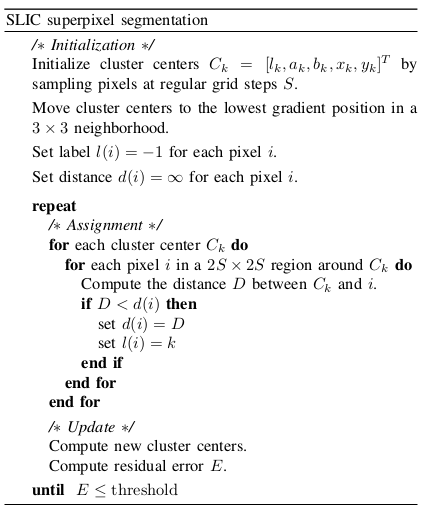
\includegraphics[width=.6\textwidth]{algoritmo_slic.png}
\caption{Algoritmo SLIC - Adaptado de \cite{SLIC}}
\label{alg:SLIC}
\end{figure}

Para o algoritmo descrito na figura \ref{alg:SLIC}, é necessário compreender o método para cálculo da medida de distância D entre os conjuntos. Devido ao algoritmo trabalhar no \textit{colorspace} CIELAB, com o espaço-plano \textit{labxy}, a posição do pixel pode assumir um intervalo de valores de acordo com o tamanho da image \ref{alg:SLIC}. Com isso, o cálculo da distância não pode ser feito utilizando uma distância euclidiana, sendo necessária uma prévia normalização da proximidade espacial e de cor. Para isso é utilizado a fórmula $D=\sqrt{d_c^2+(d_s/S)^2*m^2}$, onde $D$ corresponde a distância em 5 dimensões do espaço labxy, $d_c$ e $d_s$ correspondem à proximidade de cores e espacial; e $m^2$ corresponde a distância máxima entre cores no cluster \cite{SLIC}. Para o cálculo da distância em imagens em escala cinza, é utilizada a distância Euclidiana.

Uma etapa extra no processo de pós processamento é a união de \textit{pixels orfãos}. Esses pixels são adicionados ao cluster mais próximo usando o algoritmo de componentes conexos \cite{SLIC}.

Devido a limitação do espaço de pesquisa do algoritmo SLIC, a complexidade do algoritmo é $O(n)$, enquanto outros algoritmos que utilizam k-means para segmentação tem custo $O(k^N)$ \cite{SLIC}.

\subsection{Clusters} \label{sssec:clusters}

\subsection{Hierarquia de partições} \label{sssec:hierarchy}

\subsection{Segmentação de Imagens} \label{ssec:segmentacao}

\textit{Image segmentation is an important processing step in many image, video and computer vision applications. Extensive research has been done in creating many different approaches and algorithms for image segmentation, but it is still difficult to assess whether one algorithm produces more accurate segmentations than another, whether it be for a particular image or set of images, or more generally, for a whole class of images. To date, the most common method for evaluating the effectiveness of a segmentation method is subjective evaluation, in which a human visually compares the image segmentation results for separate segmentation algorithms, which is a tedious process and inherently limits the depth of evaluation to a relatively small number of segmentation comparisons over a predetermined set of images. Another common evaluation alternative is supervised evaluation, in which a segmented image is compared against a manually-segmented or pre-processed reference image.}

\subsection{Redes Neurais} \label{ssec:redes_neurais}


%%%%%%%%%%%%%%%%%%%%%%%%%%%%%%%%%%%%%%%%%%%%%%%%%%%%%%%
%%%%%%%%%%%%%%%%%%%%%%%%%%%%%%%%%%%%%%%%%%%%%%%%%%%%%%%
%%%%%%%%%%%%%%%%%%%%%%%%%%%%%%%%%%%%%%%%%%%%%%%%%%%%%%%

\section{Materiais e Métodos} \label{sec:mat_metodos}

%%%%%%%%%%%%%%%%%%%%%%%%%%%%%%%%%%%%%%%%%%%%%%%%%%%%%%%
%%%%%%%%%%%%%%%%%%%%%%%%%%%%%%%%%%%%%%%%%%%%%%%%%%%%%%%
%%%%%%%%%%%%%%%%%%%%%%%%%%%%%%%%%%%%%%%%%%%%%%%%%%%%%%%

\begin{figure}[ht]
\centering
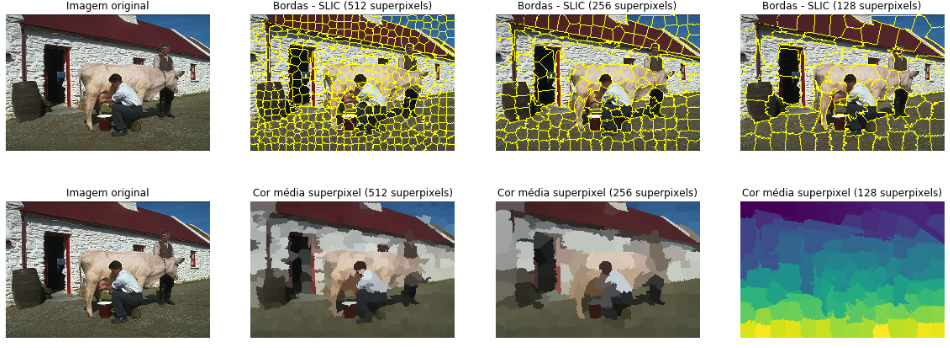
\includegraphics[width=1.\textwidth]{slic_segmentation_compare.png}
\caption{Fronteiras e coloração pelo valor médio dos superpixels SLIC/SLICO, para diferentes quantidades de superpixels}
\label{alg:SLIC}
\end{figure}


\begin{figure}[ht]
\centering
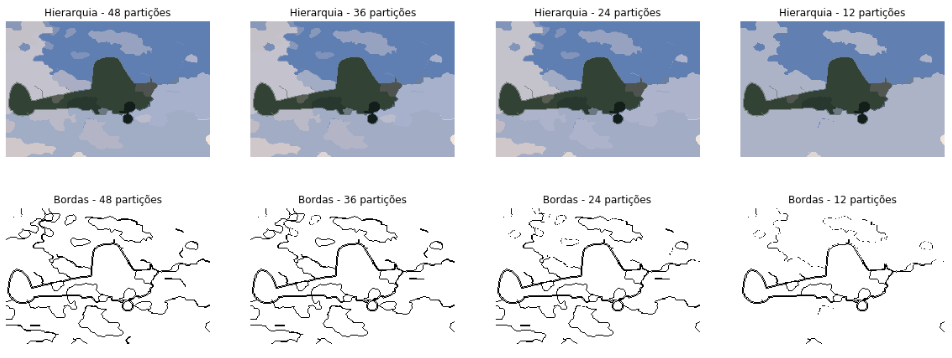
\includegraphics[width=1.\textwidth]{slic_hierarquia_particoes.png}
\caption{Fronteiras das Hierarquia de partições utilizando superpixel SLICO.}
\label{alg:SLIC}
\end{figure}


\section{Testes, Resultados e Discussões} \label{sec:testes}

%%%%%%%%%%%%%%%%%%%%%%%%%%%%%%%%%%%%%%%%%%%%%%%%%%%%%%%
%%%%%%%%%%%%%%%%%%%%%%%%%%%%%%%%%%%%%%%%%%%%%%%%%%%%%%%

\subsection{Subsections}


\begin{table}[ht]
\centering
\caption{Variables to be considered on the evaluation of interaction
  techniques}
\label{tab:exTable1}
\smallskip
\begin{tabular}{|l|c|c|}
\hline
& Value 1 & Value 2\\[0.5ex]
\hline
&&\\[-2ex]
Case 1 & 1.0 $\pm$ 0.1 & 1.75$\times$10$^{-5}$ $\pm$ 5$\times$10$^{-7}$\\[0.5ex]
\hline
&&\\[-2ex]
Case 2 & 0.003(1) & 100.0\\[0.5ex]
\hline
\end{tabular}
\end{table}

%%%%%%%%%%%%%%%%%%%%%%%%%%%%%%%%%%%%%%%%%%%%%%%%%%%%%%%
%%%%%%%%%%%%%%%%%%%%%%%%%%%%%%%%%%%%%%%%%%%%%%%%%%%%%%%
%%%%%%%%%%%%%%%%%%%%%%%%%%%%%%%%%%%%%%%%%%%%%%%%%%%%%%%

\section{Conclusão} \label{sec:conclusao}

%%%%%%%%%%%%%%%%%%%%%%%%%%%%%%%%%%%%%%%%%%%%%%%%%%%%%%%
%%%%%%%%%%%%%%%%%%%%%%%%%%%%%%%%%%%%%%%%%%%%%%%%%%%%%%%
%%%%%%%%%%%%%%%%%%%%%%%%%%%%%%%%%%%%%%%%%%%%%%%%%%%%%%%

\bibliographystyle{sbc}
\bibliography{sbc-template}

\end{document}
